\documentclass[10pt,conference,compsocconf]{IEEEtran}

\usepackage{hyperref}
\usepackage{graphicx}	% For figure environment


\begin{document}
\title{Machine Learning Report}

\author{
  Raphael Barman, Hakim Invernizzi, Rehan Mulakhel\\
  \textit{EPFL students}
}

\maketitle

\begin{figure}
\begin{center}
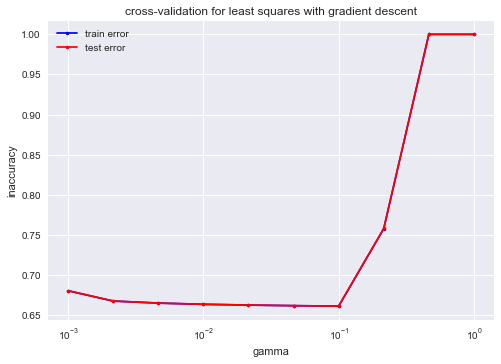
\includegraphics[width=4.5cm]{cross_validation_least_squares_GD.png}
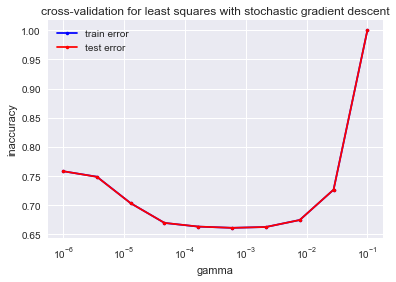
\includegraphics[width=4.5cm]{cross_validation_least_squares_SGD.png}
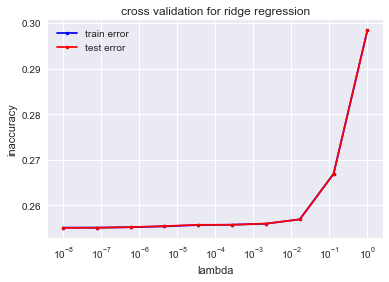
\includegraphics[width=4.5cm]{cross_validation_ridge_regression.png}
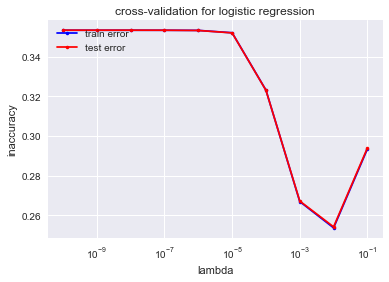
\includegraphics[width=4.5cm]{cross_validation_logistic_regression.png}
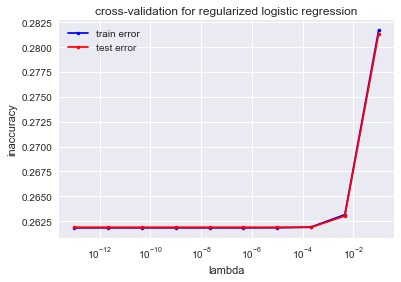
\includegraphics[width=4.5cm]{cross_validation_reg_logistic_regression.png}
 \end{center}
 \begin{center}
 \caption{\label{fig:figure1}Result of Cross-Validation with 10 folds. On the X-axis we have the ML method parameter to be tuned, on the Y-axis a measure of the inaccuracy. From top to bottom: (a) least squares GD (b) least squares SGD (c) ridge regression (d) logistic regression (e) logistic regression with regularization}
 \end{center}
\end{figure}

\section{Part I: Machine learning methods implementation}
Here is the description of our implementation of the six machine learning methods.\\
Please note that we defined our own metric to estimate prediction error, which is not the MSE but simply the percentage of uncorrectly predicted outputs, which we call inaccuracy. 
This metric is used exclusively to evaluate performance and is not part of the implementation.
 \subsection{Linear regression using gradient descent}
The implementation is simple: we iteratively update the initial weight by subtracting a pondered gradient.
Figure \ref{fig:figure1} (a) shows the cross-validation results with 500 iterations and gamma taking value in the range $[10^{-3}, 10^{0}]$ with step $10$. It can be noted that the method gives around 66\% inaccuracy in the best case, and performs best when gamma is on the order of $10^{-1}$. 
\subsection{Linear regression using stochastic gradient descent}
The difference compared to the previous method is that at each iteration the dataset is accessed at random indexes in order to
create size-1 batches. The batch gradient is then computed, pondered and used to update the weight. Figure \ref{fig:figure1} (b) shows the cross-validation results with 10000 iterations and gamma taking value in the range $[10^{-6}, 10^{-1}]$ with step $10$. it can be noted that the method also gives 66\% inaccuracy in the best case, and performs best when gamma is on the order of $10^{-3}$. 
\subsection{Least squares regression}
The pseudo-inverse of the feature matrix \textit{tx} is computed and then multiplied with the classification vector \textit{y} to obtain the weight.
The inaccuracy is of around 25.5\% for both train and test dataset.
\subsection{Ridge regression}
The weight is computed by solving the ridge regression equation, yielding $w = (X^{T}X + \lambda'I)^{-1}X^{T}y$.
Figure \ref{fig:figure1} (c) shows the cross-validation results with lambda taking value in the range $[10^{-8}, 10^{0}]$ with step $10$. It can be noted that the performance of the ridge regression is comparable to that of the simple least square regression, suggesting that regularisation applied to the whole dataset provides little improvement. This might mean that the problem is well-conditioned, or in other words that the model isn't over- nor under-fitting.
\subsection{Logistic regression}
The weight is updated by subtracting a gradient whose ponderation takes into account its hessian matrix. Figure \ref{fig:figure1} (d) shows the cross-validation results with 10000 iterations and gamma taking value in the range $[10^{-10}, 10^{-1}]$ with step $10$. It can be noted that method gives around 25.7 \% inaccuracy in the best case.
\subsection{Regularized logistic regression}
Logistic regression with the addition of a penalty term to account for linearly separable data. Figure \ref{fig:figure1} (e) shows the cross-validation results with 10000 iterations, gamma on the order of $8*10^{-3}$ and lambda taking value in the range $[10^{-10}, 10^{-1}]$ with step $10$. In can be noted that the method gives around 26.25\% inaccuracy in the best case, reinforcing what previously said about regularisation.
\section{Our Model}
\subsection{Exploratory Data Analisis and Feature Processing}
\subsubsection{Null values}
The presence of null values is well defined and allowed us to separate the
dataset in 6 groups. We noticed that all null values could be
explained by the the number of jet (PRI\_jet\_num) and by the presence or not of a
measure for the mass (DER\_mass\_MMC), thus we created 6 groups, for number of jet
$\lbrace 0, 1, 2-3 \rbrace$ and the presence or not of mass measure.

\subsubsection{Percentiles}

By looking at the 95th percentile and the maximum values of each feature, we saw
that in most cases, there were certainly a lot of outliers in some features.

\subsubsection{Histograms}

We used histograms to have an idea of the underlaying distribution.

Using the histograms, we saw that the features related to 'phi' (PRI\_tau\_phi,
PRI\_lep\_phi, PRI\_met\_phi, PRI\_jet\_leading\_phi, PRI\_jet\_subleading\_phi)
have an uniform distribution that is the same
for 'signal' and for 'background', this could mean that these features do not add
any relevant information for the classification.

We also noticed that some features (DER\_mass\_MMC, DER\_mass\_transverse\_met\_lep, DER\_mass\_vis, DER\_pt\_h, DER\_mass\_jet\_jet, DER\_pt\_tot, DER\_sum\_pt, DER\_pt\_ratio\_lep\_tau, PRI\_tau\_pt, PRI\_met, PRI\_met\_sumet, PRI\_jet\_leading\_pt, PRI\_jet\_subleading\_pt, PRI\_jet\_all\_pt) have a long tail or are exponential, thus it could be a good
idea to log-normalize theme before using them.

\subsection{ML method and Cross-validation}
We chose to use Ridge Regression as the baseline since it has the lowest
inaccuracy.
All inaccuracy results that are given have been made on a 10-fold cross validation
using Ridge Regression. The baseline, i.e. Ridge Regression on a ten-fold, is
of inaccuracy $0.255152$ with $\lambda = 10^{-10}$
We will now explore five different ways of improving the baseline.

\subsubsection{Group separation}
Using the observation we made above, we separated the dataset in 6 groups. Our
hope was that since we do not have to deal with null values, the algorithms
would find a better approximation of the underlaying distribution. We noticed an
improvement over the baseline: an inaccuracy of $0.234424$ with $\lambda =
10^{-10}$.

\subsubsection{Percentile cut}
We tried to remove all values above a certain percentile and replace them with
the percentile, in order to delete all outliers and allowing to have a less
complex model. Using the 95th percentile, we obtained an improvement: an
inaccuracy of $0.248784$ with $\lambda = 10^{-10}$

\subsubsection{Log-normalization}
Since some features had the shape of power laws and/or exponentials, we tried to
log-normalize where possible (we applied log on any value $>0$ in these
features). However, it did not result in an improvement over the baseline, with
an inaccuracy of $0.2618$ with $\lambda = 10^{-10}$. This could be explained by
the need of keeping the same distribution shape in order to be able to
differentiate 'signal' and 'background'.

\subsubsection{Removing features}
Since we noticed that the shape of all features related to 'phi' were uniforms,
we tried to remove those features in order to reduce the model complexity. We
got a slight improvement, with an inaccuracy of $0.252068$ and $\lambda =
10^{-10}$.

\subsubsection{Features augmentation}
In order to account for the model complexity, one can add some polynomial basis
to improve the fit. We obtained an improvement with a polynomial basis of degree
3: inaccuracy $= 0.229108$, $\lambda = 10^{-10}$. The improvement is quite
important, this shows that the underlying model is certainly of higher degree
than one.

\subsubsection{Final Model}
We tried different combination of the 4 improvements we found above and found
the best result with a mix of group separation, percentile cut and polynomial
basis. We found for results: inaccuracy of $0.1681$ with parameters for each groups:
$(d_0 = 7, \lambda_0 = 0)$
$(d_1 = 5, \lambda_1 = 0)$
$(d_2 = 9, \lambda_2 = 10^{-4})$
$(d_3 = 4, \lambda_3 = 1.66 \cdot 10^{-8})$
$(d_4 = 8, \lambda_4 = 4.64 \cdot 10^{-4})$
$(d_5 = 4, \lambda_5 = 0)$.

Note that until now, the usage over the Ridge Regression over least squares did
not make much sense since we always had negligible lambdas, however, with our
final model, some group benefits from the ridge regression.
\end{document}
